\documentclass{article}
\usepackage{url}
\usepackage{siunitx} % Provides the \SI{}{} command for typesetting SI units
\usepackage{graphicx} % Required for the inclusion of images
\setlength\parindent{0pt} % Removes all indentation from paragraphs
\renewcommand{\labelenumi}{\alph{enumi}.} % Make numbering in the enumerate environment by letter rather than number (e.g. section 6)
\usepackage{verbatim}
\usepackage{times} % Uncomment to use the Times New Roman font

%----------------------------------------------------------------------------------------
%	DOCUMENT INFORMATION
%----------------------------------------------------------------------------------------

\title{SFC} % Title
\author{Batman} % Author name
\date{\today} % Date for the report
\begin{document}
\maketitle % Insert the title, author and date

\begin{center}
\begin{tabular}{l r}
Date Performed: & December 31, 2013 \\ % Date the experiment was performed
Partners: & Robin \\ % Partner names
\end{tabular}
\end{center}

% If you wish to include an abstract, uncomment the lines below
% \begin{abstract}
% Abstract text
% \end{abstract}

%----------------------------------------------------------------------------------------
%	SECTION 1
%----------------------------------------------------------------------------------------

\section{Changes}

There is no significant update in SFC side.  
We only have three changes:
\begin{enumerate}
\item A new Cisco catalyst 2960 installation in SFC's NOC. 
\item A new NAT64 server based on OpenBSD-5.4-CURRENT.
\item Routing daemon updates to Quagga-0.99.22.4 in nara-gate router. 
\end{enumerate}

Because only a new NAT64 server has big significance in our operation, we will discuss in next paragraphs.  

\begin{figure}[h!]
\centering
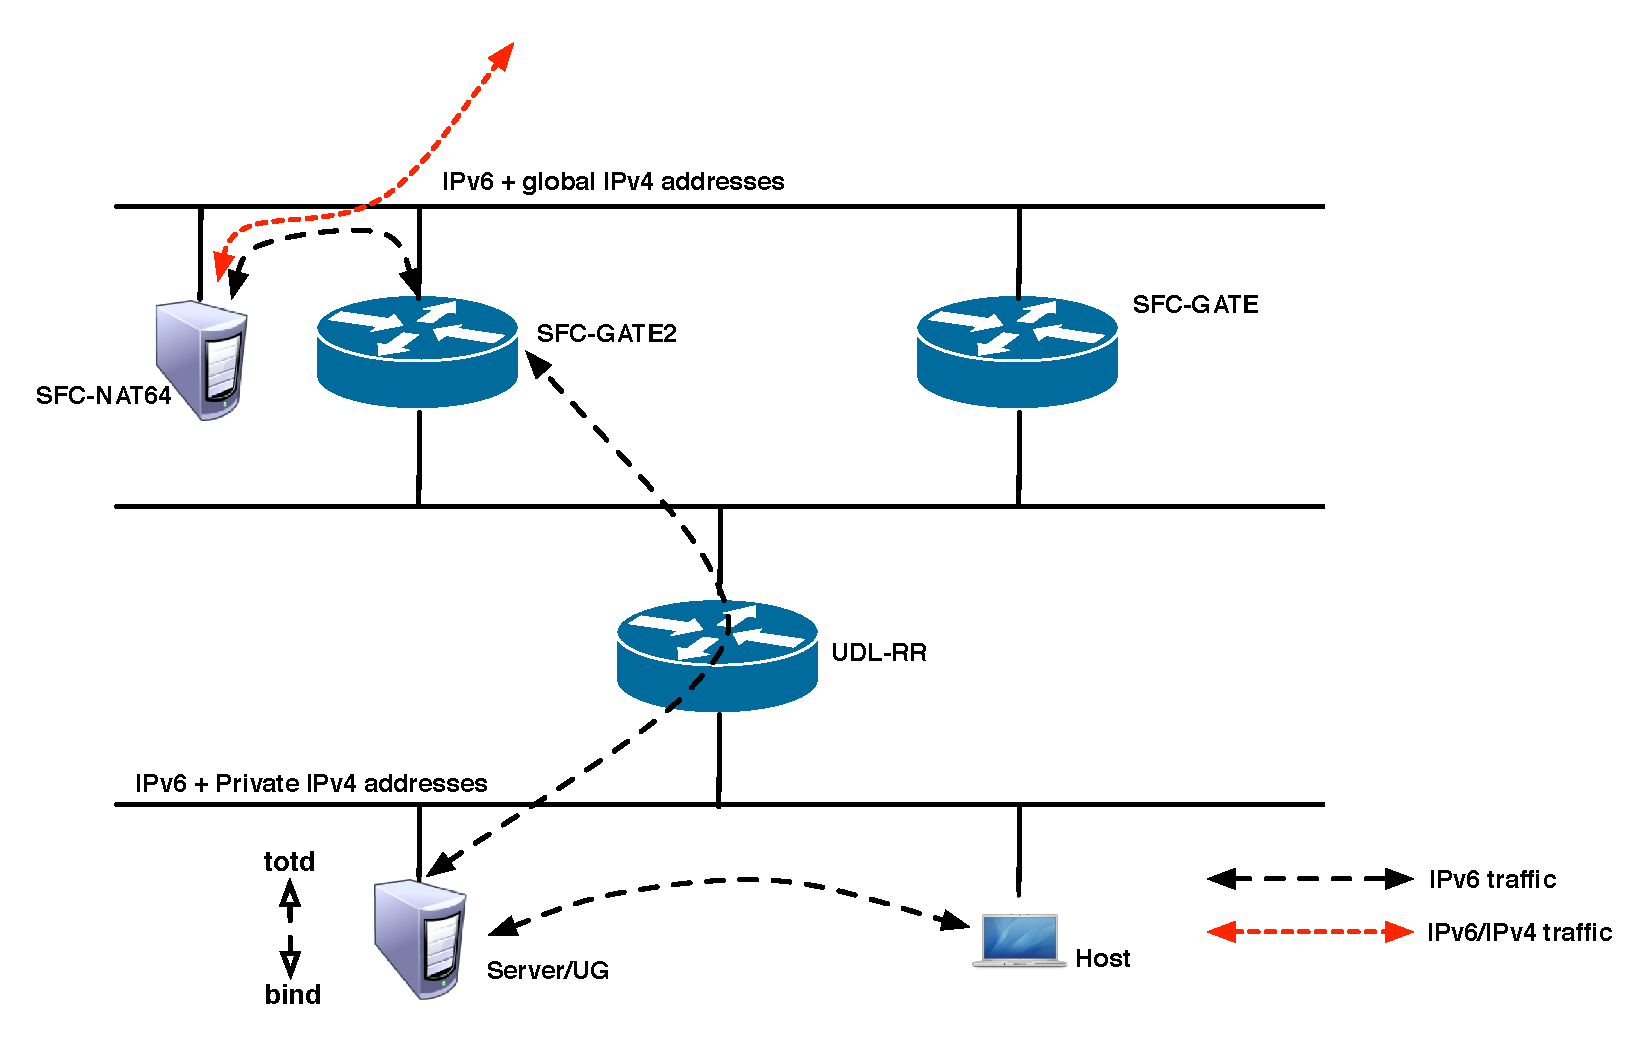
\includegraphics[width=1.\textwidth]{nat64}
\caption{Accessing IPv4 Internet via SFC-NAT64}
\label{fig:nat64}
\end{figure}

Due to un-stable of old sfc-nat64.ai3.net operation which uses naptd, we decided to change nat64 implementation from natptd to OpenBSD's nat64 implementation.  
We use OpenBSD because it is in kernel level natively support and simple configuration of translator in OpenBSD's packet filter (pf).
We also prepared backup nat64 server using Linux which uses jool kernel module from \url{https://github.com/NICMx/NAT64} in case we have trouble with OpenBSD in the future. 

Figure \ref{fig:nat64} shows how the host which has IPv6 global address and private IPv4 address can access IPv4 Internet via sfc-nat6. 
If host wants to access IPv4 website, totd daemon in server will help to translate IPv4 address of destination into IPv6 address. 
Since totd only translates IPv4 address to IPv6 address, we still need Bind for naming/DNS resolution. 
In this case totd listen in port 53 and Bind will listen on port 5353. 
AI3 uses 2001:d30:101:624::/96 IPv6 address pool for translation purpose.  
Since we added IPv6 static routing in sfc-gate2, every 2001:d30:101:624::/96 prefix will go trough sfc-nat64 and the request from server will be forwarded to sfc-nat64 server. 
Finally, sfc-nat64 server translates IPv6 address destination to IPv4 address which is last 4 bit in our  2001:d30:101:624::/96 prefix.   

An example of nat64 translation session that recorded in sfc-nat64.ai3.net is shown as follows:  
\begin{verbatim}
# pfctl -ss     
all tcp 202.249.25.29:58370 (2001:d30:112:0:2c11:f6b3:a918:6ba[37456]) -> 
   69.171.235.16:443 (2001:d30:101:624::45ab:eb10[443]) ESTABLISHED:ESTABLISHED
all tcp 202.249.25.29:56196 (2001:d30:112:0:2c11:f6b3:a918:6ba[37457]) -> 
   69.171.235.16:443 (2001:d30:101:624::45ab:eb10[443]) FIN_WAIT_2:FIN_WAIT_2
\end{verbatim}

Above session tell us that a client which has IPv6 address 2001:d30:112:0:2c11:f6b3:a918:6ba want to access IPv4 web page with IPv4 address 69.171.235.16 and port 443 (HTTP SSL).  
IPv6 address that used for translation is 2001:d30:101:624::45ab:eb10.  

\section{Publication}
In 20013, we have one publication: \\
Mohamad Dikshie Fauzie and Achmad Husni Thamrin and Jun Murai, Energy Consumption in Peer-Assisted CDN, International Journal of Advanced Research in Computer Science, vol.4, no.9, 2013.  \\

In this research we did analytical analysis of energy consumption in peer-assisted CDN, where a peer is a user that participate in a P2P network to assist content delivery.  
We presents two types of services: live streaming and online storage.  
For live streaming service, we e found that delegating workloads to peers can save up to 11% of the energy in the data center compared to the pure CDN architecture, while the savings in the total energy consumption of the system is less than 1%. For the peer-assisted online storage, we looked into several server bandwidth allocation strategies for peers of a peer-assisted online storage service and in the best case found that the energy savings of the data center and of the system are 21% and less than 2%, respectively



\end{document}
